\section{Implemented code}

Two solutions were implemented one using MPI and one using OpenMP. The MPI solution sent one image out to each core of a processor in a distributed network where as the OpenMP solution operated on a single shared-memory machine. The MPI solution had the advantage of being able to run on a series of distributed machines and so able to use more cores to complete faster. The OpenMP solution had the advantage of less overhead in the form of transferring data.

\subsection{MPI implementation}
The MPI solution worked by using the following steps.

\begin{enumerate}
	\item Create the master and n slave processes
	\item Load the psf from ./psf.bmp on the master computer
	\item Send the psf to all the slaves
	\item Get a list of all the images present on the master computer in ./Images/
	\item Send an image from the master to each of the slave processes.
	\item Each of the slaves processes the image using the Richardson-Lucy implemention.
	\item The master retrives the image from the slave and saves it to ./Output/
	\item The master sends the slave a new image
\end{enumerate}

In this implemention all the sending and receiving is done syncronsously with the exception of the retriving of the processed images from the slave. This retriving is made asyncronous so that if one of the slaves finishs faster then one that was started before it there is no delay as it waits for the slave before it to finish and send its image.

\subsection{OpenMP implementation}
The OpenMP solution worked by using the following steps.

\begin{enumerate}
	\item Load the psf from ./psf.bmp
	\item Get a list of all the images present in ./Images/
	\item load the first image
	\item run the image using the Richardson-Lucy implemention.
	\item Saves the output to ./Output/
	\item Get the next image
\end{enumerate}

The parallelization of this program occoured in two places. First during the choosing of the image to run the Richardson-Lucy algorithem on and secondly during the convolutions. The Lucy-Richardson algorithem was written so that it used a series of for loops for the convolutions rather then a convolution function (such as that provided by the CImg libraries). This meant that for each pixel and colour channel the value could be found in its own thread and combined at the end of the convolution running potentially up to 1024x1024x3 threads.

\subsection{Implementation parallisation}

In the code the data only exsits stored on one hard drive and so all the loading and saving to the hard drive could not occour in parallel. In the MPI solution as all the messages went to and from the master this was also a serial bottleneck. To find out how long these sections that would have to be executed in serial were a test was conducted. Timers were first inserted around these serial sections and then the code was set processing 16 1024 by 1024 pixel images  using a 3 by 3 psf.The computer used had a 2.0 GHz dual core processor. The results of this test can be seen summarised in Table~\ref{speed}

\begin{table}[h!]
	\caption{Parallel and serial time for code (all time in seconds)}
	\begin{center}
    	\begin{tabular}{ | l | l | l | l | l |}
    	\hline
    	 & Serial & Parallel & Total & \% Parallel  \\ \hline
		MPI & 4.71 & 386.98 & 391.69 & 98.8\% \\ \hline
		OpenMP & 2.81 & 371.45 & 374.26 & 99.7\% \\ \hline
    	\end{tabular}
	\end{center}
	\label{speed}
\end{table}

From the results it can be seen that the OpenMP implementation spent slightly less time in the serial section as was expected. Something that was not expected however was the large time reduction in the overall time of the OpenMP program with it finishing 16 seconds faster then the MPI solution. This may have been due to the extra MPI overhead or may have been caused by the optimizing compiler doing a better job with the message passing removed. From the test it was also found that each image took roughly 23 seconds to process and so to process all ten million images would require roughly 68000 hours of machine time to complete or 2833 days.

Using armdales law the speed up of the process from additional cores can be given by
\[
 \frac{1}{(1-P) + \frac{P}{S}}
\]

Where P is the amount of parrallizable code (98.9\% and 99.7\% in this case) and S is the number of processors. The amount of time in days to complete the calculation for both implementations compared to the number of cores used can be shown in Figure~\ref{mpi-time-cores}. As can be obsereved both implementations take roughly the same time. The time for one core is 2833 days, ten cores take 310 days, 20 cores take 171 days, 50 cores take 90 days and 100 cores take 58 days. Beyond this point the speed up from additional cores becomes negligible as the unparralizable sections of code take 31 days to execute. 

\begin{figure}[ht]
	\begin{center}
		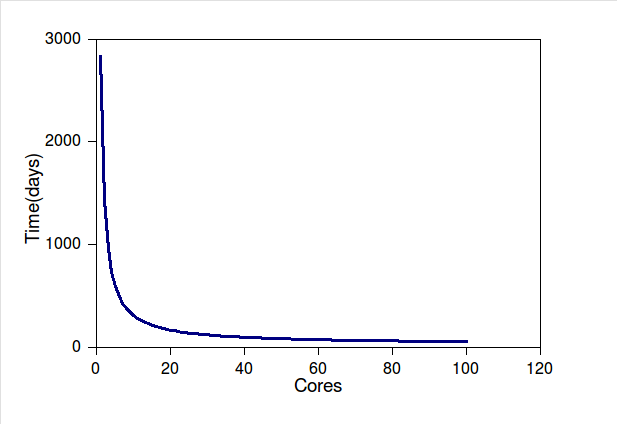
\includegraphics[width=1.0\textwidth]{mpi-time-cores}
	\end{center}
	\caption{Graph showing time to process vs number of cores for the solutions}
	\label{mpi-time-cores}
\end{figure}

For running the system the hardware required has to either be rented or brought. A desktop unit with  one 3.0 GHz quad core CPU costs around \$1000 dollars, a dual core machine costs around \$4000, a three core around \$15000 and a quad core machine costs around \$40000. For rent the Amazon EC2 service appeared to be the cheapest of the available options charging \$1.60 per hour for use of the High-CPU Extra Large Instance which provides the following 

\begin{itemize}
\item 7 GB of memory
\item 20 EC2 Compute Units (8 virtual cores with 2.5 EC2 Compute Units each)
\item 1690 GB of instance storage
\item 64-bit platform
\item I/O Performance: High (1 GigaBit ethernet)
\end{itemize}

The EC2 compute units the performance is measured in is equivalent to a 1.0-1.2 GHz 2007 Opteron or 2007 Xeon processor. These processors have roughly 60\% of the processing power of one of the test computers cores. From this information the cost of hiring and buying was calculated for a set time in which the task has to be completed. For the MPI solution both hiring amazon EC2 cores and buying multiple single CPU computers were looked at. For the OpenMP solution as shared memory was required a single machine with varing numbers of CPUs was looked at. Figure~\ref{mpi-time-money} shows the results of these calculations. Times below 40 days were not shown as the costs quickly became totally infeasible. It can be noted that for processing times longer then 100 days buying units for MPI becomes more economical then renting thanks to the one off cost rather then the cost per hour for the cpu time. It should be metioned that the cloud also offers 1 year of use for the much reduced price of \$1820.

From the graph it can be seen the shared memory element of OpenMp meant that its systems are not in the same price range as MPI and so it can be discounted as a viable solution. The full working of the equations used can be found in the appendicies

\begin{figure}[ht]
	\begin{center}
		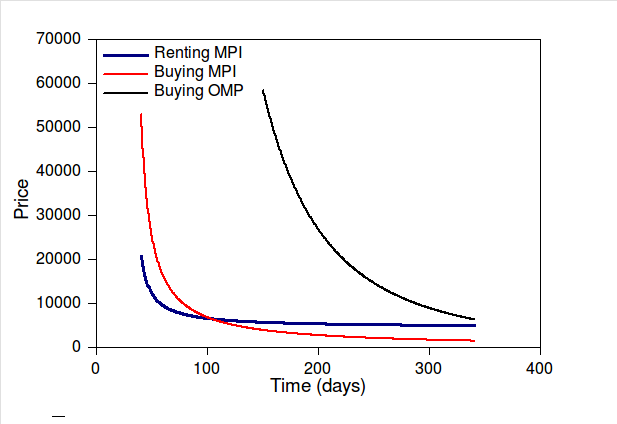
\includegraphics[width=1.0\textwidth]{mpi-time-money}
	\end{center}
	\caption{Cost comparision for the solutions taking into account time to complete}
	\label{mpi-time-money}
\end{figure}


\subsection{Cluster testing}
To see how accurate the predictions of how well the code matched up with reality the MPI code was run on a cluster. 16 1024 by 1024 pixel images were processed using 1, 2, 4, 8, 16 cores. The results can be shown in Table~\ref{shit}. The basic form of Armdales law used on the theoretical results was then applied to these results with the value for the percent of code that had to run in serial varied to give the best fit. From this a value of 96.27\% was found which fit the data with an \(r^2\) value of 0.9966 showing an exceptionally strong correlation. These points and the trend-line can be seen plotted in Figure~\ref{real_data}. These results differed slightly from the previous tests that predicted a value of 98.9\%. 

\begin{table}[h]
	\caption{Performance of code on cluster test (all times in seconds)}
	\begin{center}
    	\begin{tabular}{ | l | l |}
    	\hline
    	Cores & Run Time  \\ \hline
		1 & 473.36 \\ \hline
		2 & 231.55 \\ \hline
		4 & 140.65 \\ \hline
		8 & 61.37 \\ \hline
		16 & 36.34 \\ \hline
    	\end{tabular}
	\end{center}
	\label{shit}
\end{table}

\begin{figure}[ht]
	\begin{center}
		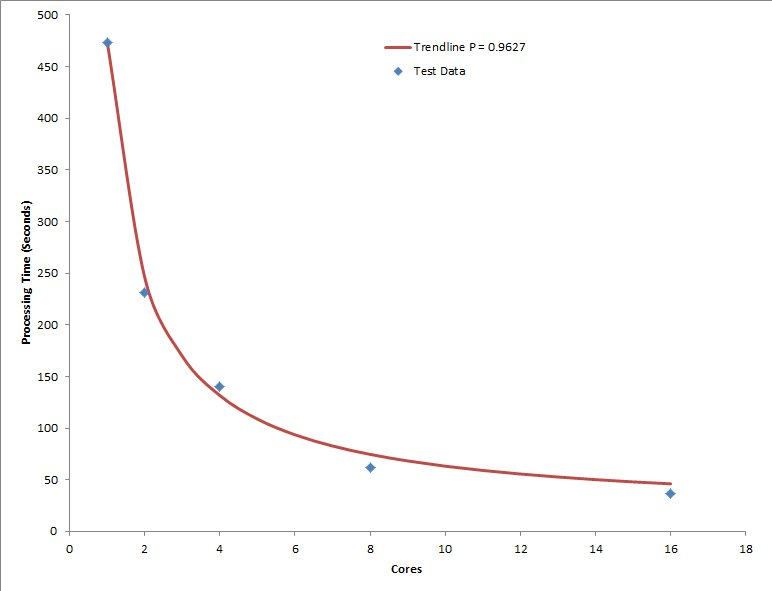
\includegraphics[width=0.7\textwidth]{Capture}
	\end{center}
	\caption{Runtime vs cores for real data}
	\label{real_data}
\end{figure}

While currently the performance of MPI code running on the cluster is slightly slower than that found to be possible by measuring IO operations I am confident that if the structure  of the MPI code was examined the causes for these slow downs that are causing the extra sections of serial execution could be found and changed so that the code could run as quickly as possible.
